% =====================================================================
%  TRANSCRIPCIÓN FIEL - EVALUACIÓN DE LA UNIDAD I (EV-PRAC-01)
%  Fundamentos de Ingeniería de Requisitos · Caso FRÍOVAC
%  Ingeniería de Requerimientos (ISR-401) · UTEQ · SPA 2026-2027
%  Compilación: pdflatex -> bibtex -> pdflatex -> pdflatex
% =====================================================================
\documentclass[11pt]{article}

\usepackage[utf8]{inputenc}
\usepackage[T1]{fontenc}
\usepackage[scaled]{helvet}
\renewcommand{\familydefault}{\sfdefault}
\usepackage[a4paper,top=2.6cm,bottom=2.3cm,left=2cm,right=2cm,headheight=34pt]{geometry}
\usepackage{graphicx}
\usepackage{array}
\usepackage{tabularx}
\usepackage{colortbl}
\usepackage{xcolor}
\usepackage{enumitem}
\usepackage{fancyhdr}
\usepackage{lastpage}
\usepackage[most]{tcolorbox}
\usepackage{amsmath}
\usepackage[numbers,sort&compress]{natbib}
\usepackage{url}
\usepackage[hypcap=false]{caption}
\usepackage[hidelinks]{hyperref}

% ---------- Textos en español ----------
\renewcommand{\tablename}{Tabla}
\renewcommand{\refname}{Referencias}

% ---------- Paleta institucional ----------
\definecolor{utegreen}{HTML}{0B7A3B}
\definecolor{utegreendk}{HTML}{075C2C}
\definecolor{midblue}{HTML}{1F5C8B}
\definecolor{gold}{HTML}{D4A017}
\definecolor{rowgray}{HTML}{EFEFEF}
\definecolor{boxgray}{HTML}{F4F6F4}
\definecolor{lightgold}{HTML}{FBF3DC}

% ---------- Columnas ----------
\newcolumntype{L}[1]{>{\raggedright\arraybackslash}p{#1}}
\newcolumntype{C}[1]{>{\centering\arraybackslash}p{#1}}
\newcolumntype{Y}{>{\raggedright\arraybackslash}X}

% ---------- Encabezado y pie ----------
\pagestyle{fancy}
\fancyhf{}
\lhead{\footnotesize UTEQ \,$\cdot$\, Ingeniería de Requerimientos (ISR-401) \,$\cdot$\, SPA 2026--2027}
\rhead{\footnotesize EV-PRAC-01 \,$\cdot$\, Unidad I}
\lfoot{\footnotesize Transcripción fiel --- Caso «FRÍOVAC»}
\rfoot{\footnotesize Página \thepage\ de \pageref{LastPage}}
\renewcommand{\headrulewidth}{0.6pt}
\renewcommand{\footrulewidth}{0.4pt}

\setlength{\parindent}{0pt}
\setlength{\parskip}{5pt}
\setlength{\emergencystretch}{3em}
\renewcommand{\arraystretch}{1.25}

% ---------- Atajos ----------
\newcommand{\thdr}[1]{\cellcolor{utegreen}\textcolor{white}{\textbf{#1}}}
\newcommand{\bhdr}[1]{\cellcolor{midblue}\textcolor{white}{\textbf{#1}}}
\newcommand{\seccion}[1]{\section{\textcolor{utegreendk}{#1}}}

\newtcolorbox{cajaaviso}[1][]{colback=lightgold,colframe=gold!80!black,boxrule=0.8pt,arc=2mm,fonttitle=\bfseries,breakable,#1}
\newtcolorbox{cajatarea}[1][]{colback=white,colframe=midblue,boxrule=0.7pt,arc=1.5mm,fonttitle=\bfseries,coltitle=white,colbacktitle=midblue,breakable,#1}

\begin{document}

% =====================================================================
% ENCABEZADO Y DATOS DE IDENTIFICACIÓN
% =====================================================================
\begin{center}
	{\large Facultad de Ciencias de la Computación \,$\cdot$\, Carrera de Software}\\[6pt]
	{\LARGE\textbf{\textcolor{utegreendk}{EVALUACIÓN DE LA UNIDAD I (EV-PRAC-01)}}}\\[4pt]
	{\large Fundamentos de Ingeniería de Requisitos --- Caso «FRÍOVAC»}
\end{center}
\noindent\textcolor{gold}{\rule{\linewidth}{1.5pt}}

\vspace{4pt}
\noindent\begin{tabularx}{\linewidth}{|L{0.30\linewidth}|Y|}
	\hline
	\bhdr{Apellidos y nombres} & Frixon Morán\\
	\hline
	\bhdr{Asignatura} & Ingeniería de Requerimientos (ISR-401) --- 4.\textsuperscript{o} nivel, paralelo A\\
	\hline
	\bhdr{Docente} & Gleiston Cicerón Guerrero Ulloa, PhD\\
	\hline
	\bhdr{Fecha} & 18 de noviembre de 2026\\
	\hline
\end{tabularx}

\vspace{6pt}
\begin{cajaaviso}[title={Declaración de transcripción fiel (Regla R5)}]
	Esta es la transcripción fiel de la prueba escrita a mano el 18 de noviembre de 2026; las fotografías de las hojas están en el anexo.
\end{cajaaviso}

% =====================================================================
\seccion{Desarrollo de Tareas}
% =====================================================================

\begin{cajatarea}[title={T1. Conceptos aplicados al caso \hfill D1 · 10\,\%}]
	\textbf{(a) Definición de requisito según ISO/IEC/IEEE 29148:2018 \citep{iso29148_2018} y análisis de E7 y E12:}\\
	Un requisito se define según ISO/IEC/IEEE 29148:2018 \citep{iso29148_2018} una condición que necesita un usuario para resolver un problema o alcanzar un objetivo.
	\begin{itemize}[leftmargin=18pt,itemsep=2pt]
		\item \textbf{E7} No es un requisito del producto, es un enunciado descriptivo del procedimiento actual. (SWEBOK v4.0, cap. 1 \citep{swebok_v4_2024}).
		\item \textbf{E12} No es un requisito del producto, sino una restricción o condición de gestión del proyecto (SWEBOK v4.0, cap. 1 \citep{swebok_v4_2024}).
	\end{itemize}

	\textbf{(b) Perspectiva de sistemas (StRS, SyRS y SRS) según ISO/IEC/IEEE 29148:2018 \citep{iso29148_2018}:}
	\begin{itemize}[leftmargin=18pt,itemsep=2pt]
		\item \textbf{StRS (Stakeholder Requirements Specification):} Describe las necesidades, expectativas y restricciones de los interesados desde la perspectiva de negocio y uso (29148, 2018 \citep{iso29148_2018}). \emph{Enunciado del Insumo A:} \textbf{E1} («Necesitamos enterarnos de inmediato\ldots»), porque refleja directamente la necesidad crítica de la coordinadora de inmunizaciones.
		\item \textbf{SyRS (System Requirements Specification):} Describe las capacidades técnicas, interfaces y comportamiento del sistema global (hardware + software + actores humanos) (29148, 2018 \citep{iso29148_2018}). \emph{Enunciado del Insumo A:} \textbf{E3} («El sensor TL-40\ldots envía una lectura cada 10 minutos usando el protocolo MQTT»), ya que especifica el comportamiento técnico del hardware del sistema global.
		\item \textbf{SRS (Software Requirements Specification):} Describe de forma exclusiva los requisitos funcionales y no funcionales asignados al componente de software (29148, 2018 \citep{iso29148_2018}). \emph{Enunciado del Insumo A:} \textbf{E5} («El sistema generará en formato PDF el informe mensual\ldots»), porque define una función automatizada propia de la plataforma de software.
	\end{itemize}

	\textbf{(c) Actividades del proceso de IR (SWEBOK v4.0, cap. 1 \citep{swebok_v4_2024}) y marco de Pohl \citep{pohl_2025} (H1 a H5):}
	\begin{itemize}[leftmargin=18pt,itemsep=2pt]
		\item \textbf{H1:} Actividad de \textbf{Elicitación} --- Tipo \textbf{Central} (según el marco de Pohl \citep{pohl_2025}).
		\item \textbf{H2:} Actividad de \textbf{Análisis y negociación} --- Tipo \textbf{Central} (según el marco de Pohl \citep{pohl_2025}).
		\item \textbf{H3:} Actividad de \textbf{Especificación} --- Tipo \textbf{Central} (según el marco de Pohl \citep{pohl_2025}).
		\item \textbf{H4:} Actividad de \textbf{Validación} --- Tipo \textbf{Central} (según el marco de Pohl \citep{pohl_2025}).
		\item \textbf{H5:} Actividad de \textbf{Gestión (de requisitos/cambios)} --- Tipo \textbf{Transversal} (según el marco de Pohl \citep{pohl_2025}).
	\end{itemize}
\end{cajatarea}

\begin{cajatarea}[title={T2. Clasificación y auditoría \hfill D2 · 30\,\%}]
	\textbf{(a) Clasificación de Insumo A (E1 a E12)}

	\vspace{4pt}
	{\small
	\noindent\begin{tabularx}{\linewidth}{|C{0.07\linewidth}|L{0.24\linewidth}|L{0.20\linewidth}|Y|}
		\hline
		\thdr{ID} & \thdr{Tipo} & \thdr{Documento} & \thdr{Justificación}\\
		\hline
		E1 & Funcional & SRS / SyRS & Define la capacidad del sistema de notificar excursiones térmicas de inmediato (29148, 2018 \citep{iso29148_2018}).\\
		\hline
		\rowcolor{rowgray} E2 & Requisito de dominio & StRS / SyRS & Norma técnica obligatoria sobre los rangos de conservación de vacunas (+2\,°C a +8\,°C) (SWEBOK v4.0, cap. 1 \citep{swebok_v4_2024}).\\
		\hline
		E3 & Requisito de dominio / Restricción técnica & SyRS & Especificación fija de operación del hardware adquirido (sensor TL-40 y MQTT) (29148, 2018 \citep{iso29148_2018}).\\
		\hline
		\rowcolor{rowgray} E4 & Restricción (plazo y presupuesto) & StRS & Límite innegociable de fecha de entrega (30/06/2027) y costo máximo (USD 48\,000) (29148, 2018 \citep{iso29148_2018}).\\
		\hline
		E5 & Funcional & SRS & El sistema genera de forma automatizada el informe mensual de temperaturas (29148, 2018 \citep{iso29148_2018}).\\
		\hline
		\rowcolor{rowgray} E6 & Funcional (con condición operativa) & SyRS / SRS & Define el registro continuo de datos ante cortes eléctricos de hasta 8 horas (29148, 2018 \citep{iso29148_2018}).\\
		\hline
		E7 & No es requisito & Ninguno (Bitácora / Contexto) & Describe únicamente el procedimiento manual actual de control de temperatura (SWEBOK v4.0, cap. 1 \citep{swebok_v4_2024}).\\
		\hline
		\rowcolor{rowgray} E8 & No funcional (Eficiencia de desempeño - Capacidad) & SRS & Establece un umbral estricto de rendimiento ($<$ 3\,s con 50 usuarios concurrentes) (ISO/IEC 25010:2023 \citep{iso25010_2023}).\\
		\hline
		E9 & Restricción (Plataforma tecnológica) & SRS & Impone el despliegue obligatorio de la plataforma en servidores Linux del distrito (29148, 2018 \citep{iso29148_2018}).\\
		\hline
		\rowcolor{rowgray} E10 & Funcional + Seguridad (Protección) & SRS & Establece control de acceso por roles y trazabilidad de autoría en acciones correctivas (ISO/IEC 25010:2023 \citep{iso25010_2023}).\\
		\hline
		E11 & No funcional (Capacidad de interacción / Usabilidad) & SRS & Define una métrica de aprendizaje y efectividad de uso ($<$ 2\,min en 1er intento) (ISO/IEC 25010:2023 \citep{iso25010_2023}).\\
		\hline
		\rowcolor{rowgray} E12 & No es requisito & Ninguno (Gestión de proyecto) & Establece una directriz logística y organizativa para la planificación del proyecto (SWEBOK v4.0, cap. 1 \citep{swebok_v4_2024}).\\
		\hline
	\end{tabularx}
	}

	\vspace{8pt}
	\textbf{(b) Auditoría del Insumo B (B1 a B6)}

	\vspace{4pt}
	{\small
	\noindent\begin{tabularx}{\linewidth}{|C{0.06\linewidth}|L{0.21\linewidth}|L{0.21\linewidth}|L{0.15\linewidth}|Y|}
		\hline
		\thdr{ID} & \thdr{Término o construcción problemática} & \thdr{Característica de 29148 que incumple} & \thdr{Propiedad SMART que incumple} & \thdr{Justificación}\\
		\hline
		B1 & «rápido y fácil de usar» & \emph{Unambiguous} (no ambigüedad), \emph{Verifiable} (verificable) y \emph{Singular} (29148, 5.2.5 \citep{iso29148_2018}) & \emph{Specific} y \emph{Measurable} \citep{mannion_smart_1995} & Mezcla múltiples cualidades subjetivas sin métricas ni umbrales que permitan probar objetivamente su cumplimiento (29148, 5.2.5 \citep{iso29148_2018}).\\
		\hline
		\rowcolor{rowgray} B2 & «alertas oportunas» e «inadecuada» & \emph{Unambiguous} y \emph{Verifiable} (29148, 5.2.5 \citep{iso29148_2018}) & \emph{Measurable} \citep{mannion_smart_1995} & Emplea términos vagos sin definir plazos máximos («oportunas») ni umbrales térmicos exactos («inadecuada») (29148, 5.2.5 \citep{iso29148_2018}).\\
		\hline
		B3 & «en todo momento, incluso sin energía ni conexión, indefinidamente» & \emph{Feasible} (factible / realizable) y \emph{Consistent} (29148, 5.2.5 \citep{iso29148_2018}) & \emph{Attainable} (alcanzable) \citep{mannion_smart_1995} & Exige autonomía y almacenamiento infinitos, lo cual es físicamente imposible y contradice el límite de 8 horas del caso (E6) (29148, 5.2.5 \citep{iso29148_2018}).\\
		\hline
		\rowcolor{rowgray} B4 & «base de datos MongoDB alojada en la nube de AWS» & \emph{Implementation-free} (libre de diseño prematuro) (29148, 5.2.5 \citep{iso29148_2018}) & \emph{Realisable} (en contexto) \citep{mannion_smart_1995} & Impone decisiones tecnológicas específicas de arquitectura sin justificación funcional y contradice la restricción E9 (29148, 5.2.5 \citep{iso29148_2018}).\\
		\hline
		B5 & «Si es posible\ldots exportar los datos a Excel, CSV, etc.» & \emph{Unambiguous}, \emph{Complete} y criterios de lenguaje condicional y lista abierta «etc.» (29148, 5.2.3 / 5.2.5 / 5.2.7 \citep{iso29148_2018}) & \emph{Specific} \citep{mannion_smart_1995} & El condicional «Si es posible» elimina la obligatoriedad (\emph{debe}) y «etc.» deja los formatos de salida indefinidos (29148, 5.2.7 \citep{iso29148_2018}).\\
		\hline
		\rowcolor{rowgray} B6 & \emph{Ninguno (Requisito bien formado)} & Cumple la construcción formal de \textbf{29148, 5.2.4} \citep{iso29148_2018} & Cumple todas las propiedades SMART \citep{mannion_smart_1995} & Presenta estructura completa: condición, sujeto, verbo modal obligatorio (\texttt{deberá enviar}), objeto y restricción medible (29148, 5.2.4 \citep{iso29148_2018}).\\
		\hline
	\end{tabularx}
	}
\end{cajatarea}

\begin{cajatarea}[title={T3. Redacción de requisitos bien formados (hasta B5) \hfill D3 · 30\,\%}]
	\emph{(Estructura aplicada según ISO/IEC/IEEE 29148:2018, cláusula 5.2.4 \citep{iso29148_2018}: [Condición] [Sujeto] [Acción] [Objeto] [Restricción de la acción])}

	\vspace{4pt}
	{\small
	\noindent\begin{tabularx}{\linewidth}{|C{0.07\linewidth}|Y|L{0.18\linewidth}|C{0.09\linewidth}|L{0.10\linewidth}|L{0.11\linewidth}|}
		\hline
		\thdr{ID} & \thdr{Enunciado} & \thdr{Tipo (ISO/IEC 25010:2023 \citep{iso25010_2023})} & \thdr{Doc.} & \thdr{Fuente} & \thdr{Método de verif.}\\
		\hline
		B1a & Cuando un usuario solicite consultar el historial de temperaturas de un establecimiento, el sistema debe mostrar los registros en pantalla en un tiempo máximo de 3 segundos con hasta 50 usuarios concurrentes. & No funcional (Eficiencia de desempeño \citep{iso25010_2023}) & SRS & B1, E8 & Prueba\\
		\hline
		\rowcolor{rowgray} B1b & Cuando un responsable de vacunatorio sin capacitación previa utilice la aplicación móvil por primera vez, el sistema debe permitir completar el registro de una acción correctiva en un tiempo no mayor a 2 minutos. & No funcional (Capacidad de interacción \citep{iso25010_2023}) & SRS & B1, E11 & Demostración\\
		\hline
		B2 & Cuando el sensor TL-40 registre una temperatura inferior a +2,0\,°C o superior a +8,0\,°C, el sistema debe enviar una notificación de alerta por SMS al responsable del vacunatorio y a la coordinadora distrital en un plazo máximo de 5 minutos. & Funcional (Adecuación funcional \citep{iso25010_2023}) & SRS & B2, E1, E2, B6 & Prueba\\
		\hline
		\rowcolor{rowgray} B3 & Cuando ocurra una interrupción del suministro eléctrico o de la red celular en un establecimiento, el sensor TL-40 debe almacenar localmente las lecturas de temperatura tomadas cada 10 minutos durante un período continuo de hasta 8 horas. & No funcional (Fiabilidad \citep{iso25010_2023}) & SyRS & B3, E3, E6 & Prueba\\
		\hline
		B5 & Cuando la coordinadora de inmunizaciones solicite el consolidado de temperaturas de los 16 establecimientos, el sistema debe exportar el reporte en formatos PDF y CSV en un tiempo máximo de 10 segundos. & Funcional (Adecuación funcional \citep{iso25010_2023}) & SRS & B5, E5 & Demostración\\
		\hline
	\end{tabularx}
	}
\end{cajatarea}

% =====================================================================
% BIBLIOGRAFÍA (Generada desde referencias.bib)
% =====================================================================
\bibliographystyle{plainnat}
\bibliography{referencias}

% =====================================================================
% ANEXO DE FOTOGRAFÍAS (Reglas R1 - R5)
% =====================================================================
\newpage
\seccion{Anexo: Evidencias fotográficas de la prueba escrita}

\begin{center}
    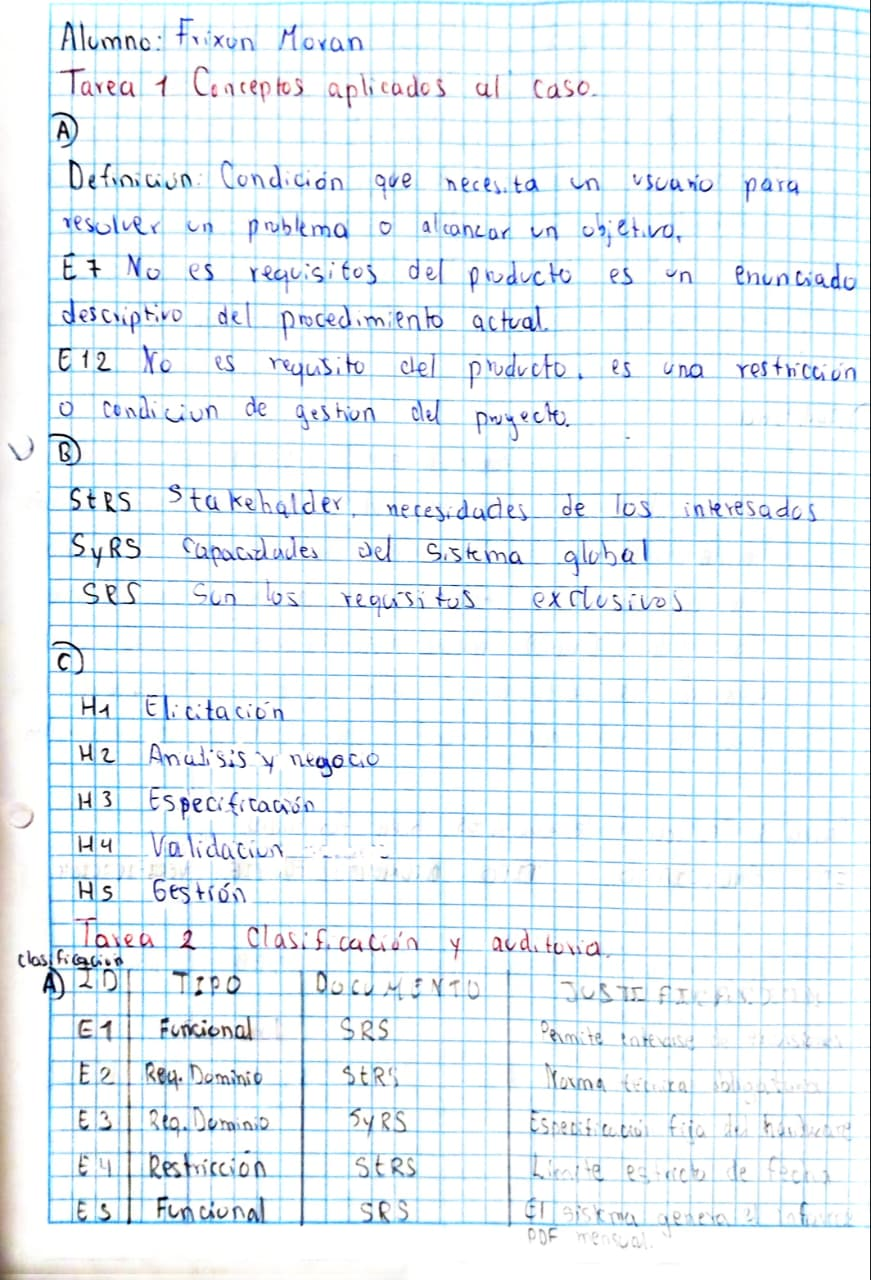
\includegraphics[width=0.85\textwidth]{evidencias/hoja-01.jpg}\\[12pt]
    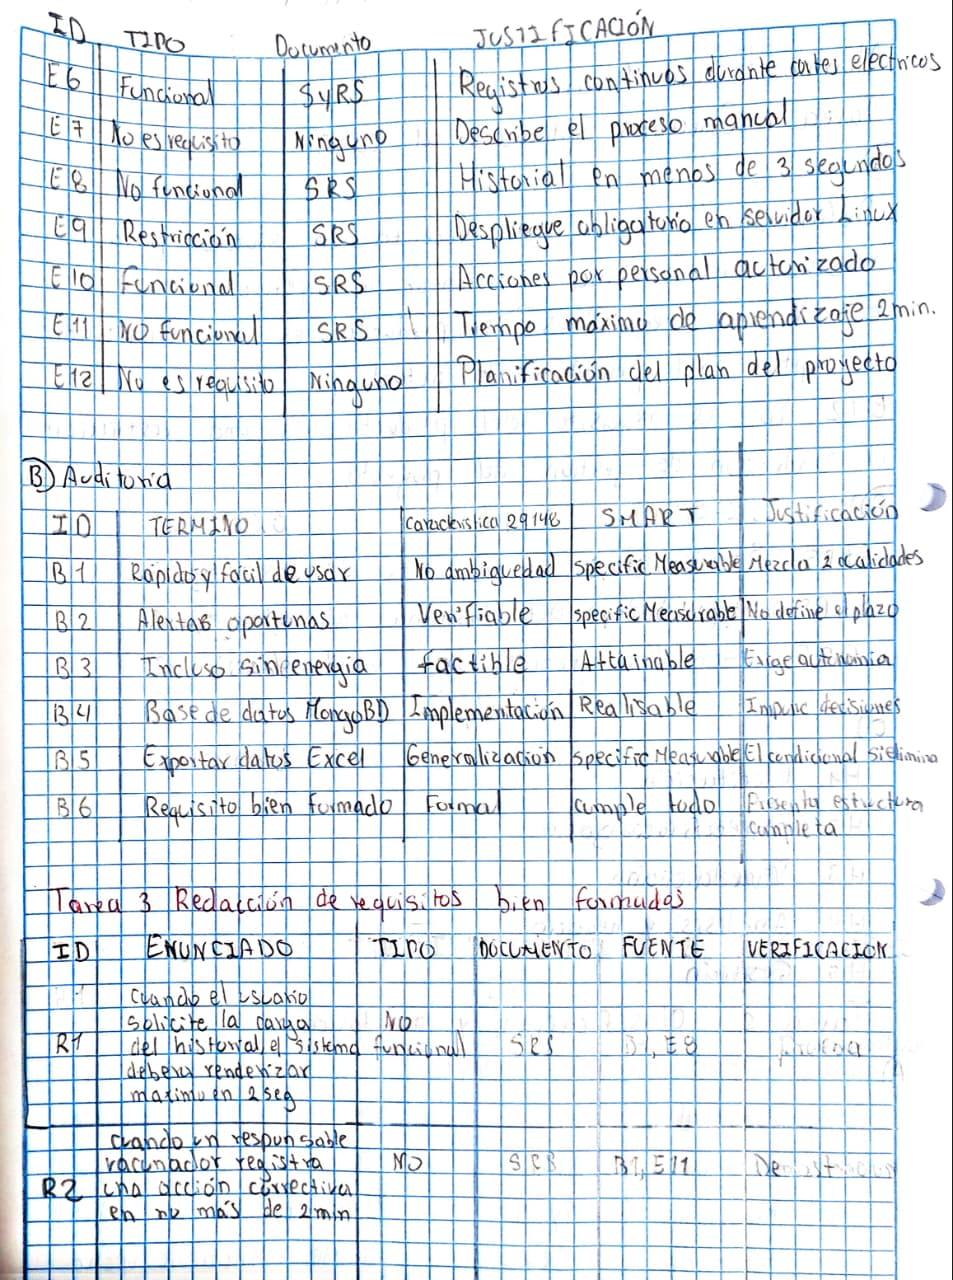
\includegraphics[width=0.85\textwidth]{evidencias/hoja-02.jpg}\\[12pt]
    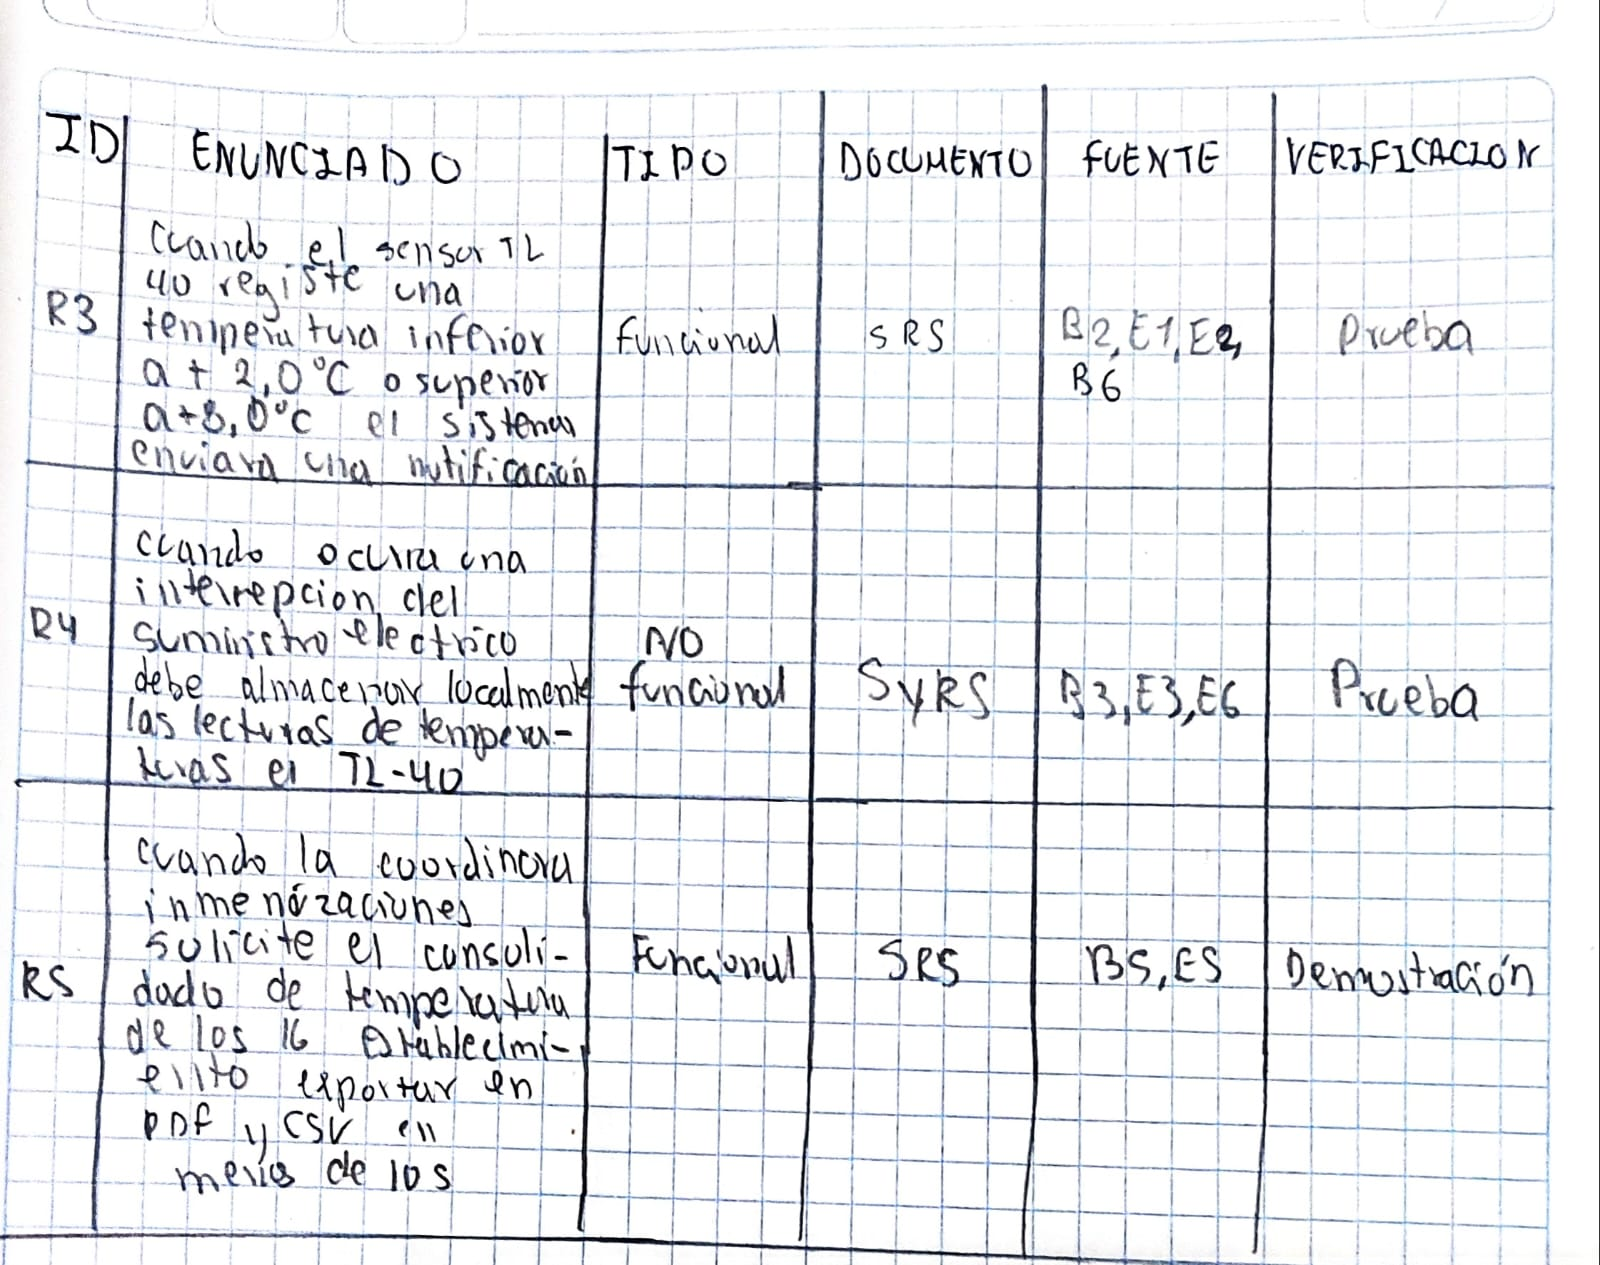
\includegraphics[width=0.85\textwidth]{evidencias/hoja-03.jpg}
\end{center}

\end{document}
